\section{Discussion}
\label{sec:discussion}
In this section, we first evaluate the importance of each relational view for our boosted model. We then compare with approaches proposed to merge neural networks in general in other domains. We then illustrate \emph{discriminative magnification effect} in detail and study the robustness of our model to training label sparsity.  We also extend our proposed approach to include textual features and compare it with a text-based model. Finally, we provide a theoretical analysis of performance gains of our Contrastive GCN model and provide limitations of our approach.

\subsection{Ablation Study on Relation Types}
\begin{table}[h]
 \centering
  \robustify\bfseries
  \begin{tabular}{l | c | c| c| c|c | c}
    \toprule
       {\{ Relation Type\}} &
        {Tech} &
        {Culture} &
        {Life} &
        {Sci}&
        {Business} & {AskDocs}\\
      \midrule
      C & 71.23 &75.90 &78.71&72.99 & 76.85 & 67.39\\
    \{ TS, AS \} & 67.86 &74.15 &75.75&65.80& 76.13 & 84.57 \\
    R & 68.30 & 73.35 & 76.57 & 67.40 & 75.76 & 62.30\\
    \{TS, AS \} + R & 69.28 & 75.50 &76.41 &70.11 &77.90 & 86.34  \\
    C + R & 73.04 & 77.66 & 80.25 &73.72 & 80.04 & 70.02\\
    C + \{ TS, AS \} & 72.81 & 78.04 & 81.41 & 72.19 & 80.15 & 86.99\\
    C + \{ TS, AS \} + R & \bfseries 73.87 & \bfseries 78.74 & \bfseries 81.60&  \bfseries74.68&  \bfseries80.56 & \bfseries 87.60\\
    \bottomrule
  \end{tabular}
  \caption{\label{tab:relation} 5-fold Accuracy (in \%) comparison for different combination of relation types for our boosted model. Contrastive and Similar Contrast relations together performs similar to the final model.}
\end{table}
We present results of an ablation study with different combination of relation types (Contrastive, Similar and Reflexive) used for IR-GCN model in Table \ref{tab:relation}. We conducted this study on the biggest community from each of the five categories, i.e., ServerFault (Technology), English (Culture), Science Fiction (Life), Physics (Science), Workplace (Business). We also report results for AskDocs subreddit.
Similar Contrast relation (TrueSkill and Arrival) used in isolation perform the worst among all the variants. Training Contrastive and Similar Contrast relation together in our boosted framework performs similar to our final model. Reflexive GCN contributes the least as it does not consider any neighbors.

\subsection{Aggregator Architecture Variants}
\label{sec:agg}
We compare our gradient boosting based aggregation approach with other popular methods used in literature to merge different neural networks discussed in \cref{item:aggregator}.
\begin{table}[h]
  %\small
  \centering
  \robustify\bfseries
  \begin{tabular}{l | c | c| c| c|c|c}
    \toprule
    {Method} &
    {Tech} &
    {Culture} &
    {Life} &
    {Sci}&
    {Business} & {AskDocs}\\
      \midrule
    Stacking~\cite{Stacking} &68.58 & 74.44 & 79.19 & 70.29 &75.50 & 85.40 \\
    Fusion~\cite{Fusion18}  &72.30 &77.25 & 80.79 & 73.91 &79.01 & 86.33\\
    NeighborAgg~\cite{graphsage, relationalGCN}  &69.29 &74.28 & 77.94 & 68.42 &78.64 & 86.00  \\
    IR-GCN & \bfseries 73.87 & \bfseries 78.74 & \bfseries 81.60&  \bfseries74.78&  \bfseries80.56 & \bfseries 87.60\\
    \bottomrule
  \end{tabular}
  \caption{\label{tab:agg} 5-fold Accuracy (in \%) comparison of different aggregator architectures. These architectures perform worse than Contrastive GCN for StackExchange. Fusion performs similarly but is computationally expensive.}
\end{table}

Table \ref{tab:agg} reports the accuracy results for these aggregator variants as compared to our model. Our method outperforms all the variants with Fusion performing the best.  This superior performance affirms that existing aggregation models are not suitable for our problem. Note that these approaches perform worse than even Contrastive GCN except Fusion. The fusion approach performs similarly to our approach but is computationally expensive as the input size for each view is linear in the number of all views in the model.

\subsection{Discriminative Magnification effect}

\begin{figure}[tbh]
  \centering
  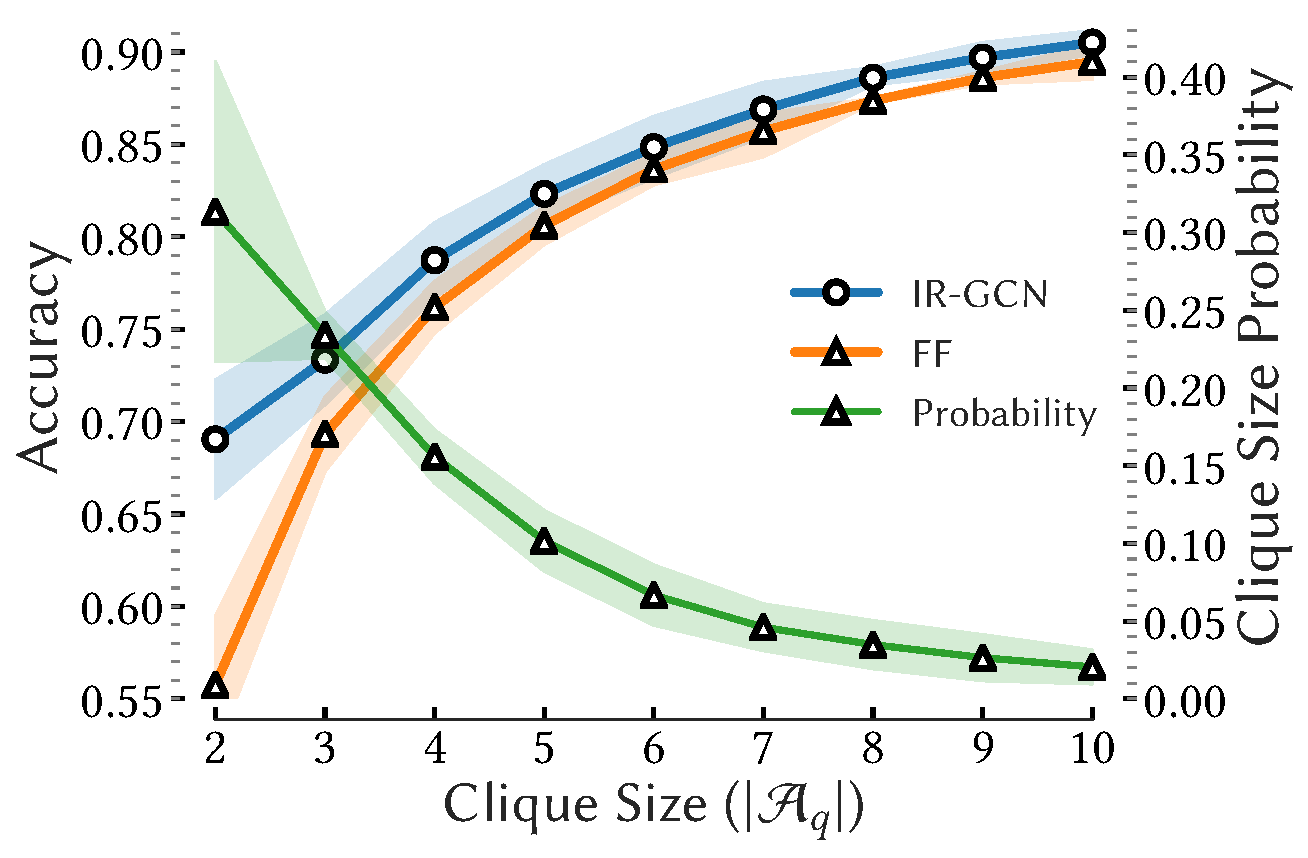
\includegraphics[scale=0.5]{figures/clique_acc.pdf}
  \caption{\label{fig:clique} Accuracy of our IR-GCN model compared to the FF model with varying clique size (i.e. number of answers to a question, $\vert \mathcal{A}_q \vert$) for Contrastive view .
We report averaged results over the largest community of all categories. Our model performs much better for smaller cliques, and the effect diminishes for larger cliques (\cref{eq:contrast}). 80\% of the questions have $< 4$ answers.}
\end{figure}

We show that due to our proposed modification to the convolution operation for contrastive view, we achieve \emph{Discriminative Magnification effect} (\cref{eq:contrast}). Note that the difference is scaled by Clique size ($1 + 1/n-1$), i.e. number of answers to a question, $\vert \mathcal{A}_q \vert$. Figure \ref{fig:clique} shows the accuracy of our IR-GCN model as compared to the FeedForward model with varying clique size. Recall that the FeedForward model predicts node labels independent of other nodes and is not affected by clique size. We report average results over the same five communities as above. We can observe that increase in accuracy is much more for lower clique sizes (13\% improvement for $\vert \mathcal{A}_q \vert = 2$ and 4\% for $\vert \mathcal{A}_q \vert = 3$ on average). The results are almost similar for larger clique sizes. In other words, our model significantly outperforms the FeedForward model for questions with fewer candidate answers. However, around 80\% of the questions have very few answers($< 4$), and thus this gain over FF is significant.

\begin{figure}[h]
      \centering
  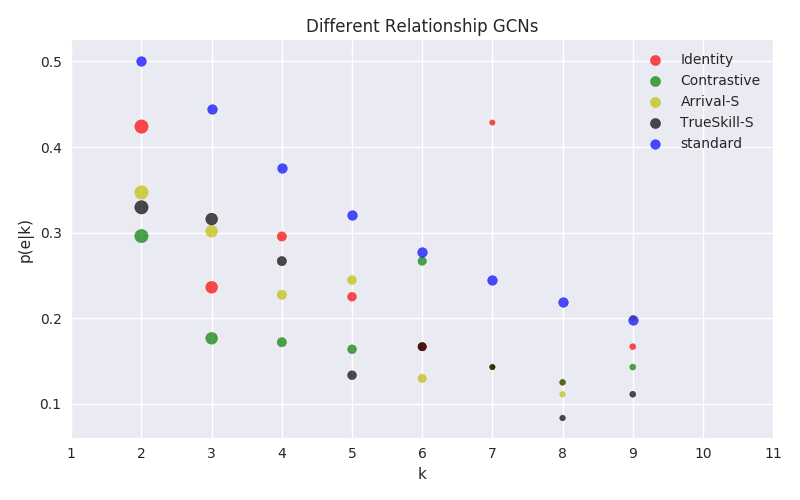
\includegraphics[scale=0.55]{figures/ErrorPlot.png}
  \caption{\label{fig:error} Probability of error with varying clique size for movie StackExchange. Standard represents random selection. Contrastive view outperforms other views for smaller clique sizes.  }
\end{figure}

Alternatively, we also plot the probability of error per tuple given each clique size ($p(e|k)$) for the movie StackExchange in \Cref{fig:error}. The \emph{standard} corresponds to a naive baseline of randomly selecting an accepted answer within each clique. For this standard baseline, error probability per clique can be denoted as,
\begin{align}
p(e|k) = (1 - 1/k) * \frac{2}{k} = \frac{2(k-1)}{k^2}
\end{align}
$(1 - 1/k)$ denotes the probability of choosing the wrong accepted answer, while $2/k$ is the actual error rate in these scenarios. The error rate is such because even in cases where the baseline chose the wrong accepted answer, remaining answers are still correctly classified as not accepted. Thus, there are only two errors per clique.

The standard baseline performs the worst as the error probability is highest than the other baselines for each clique. The Contrastive view has the least error probability for smaller cliques ($k<5$). This result is analogous to the performance gain illustrated above due to the \emph{Discriminative Magnification effect}. For larger cliques, similar contrast views (ArrivalSkill and TrueSkill) have the least error probability. As both of these views connects similar tuples across different questions, they are thus more useful for questions with a higher number of competing answers.



\subsection{Label Sparsity}

\begin{figure}[h]
      \centering
  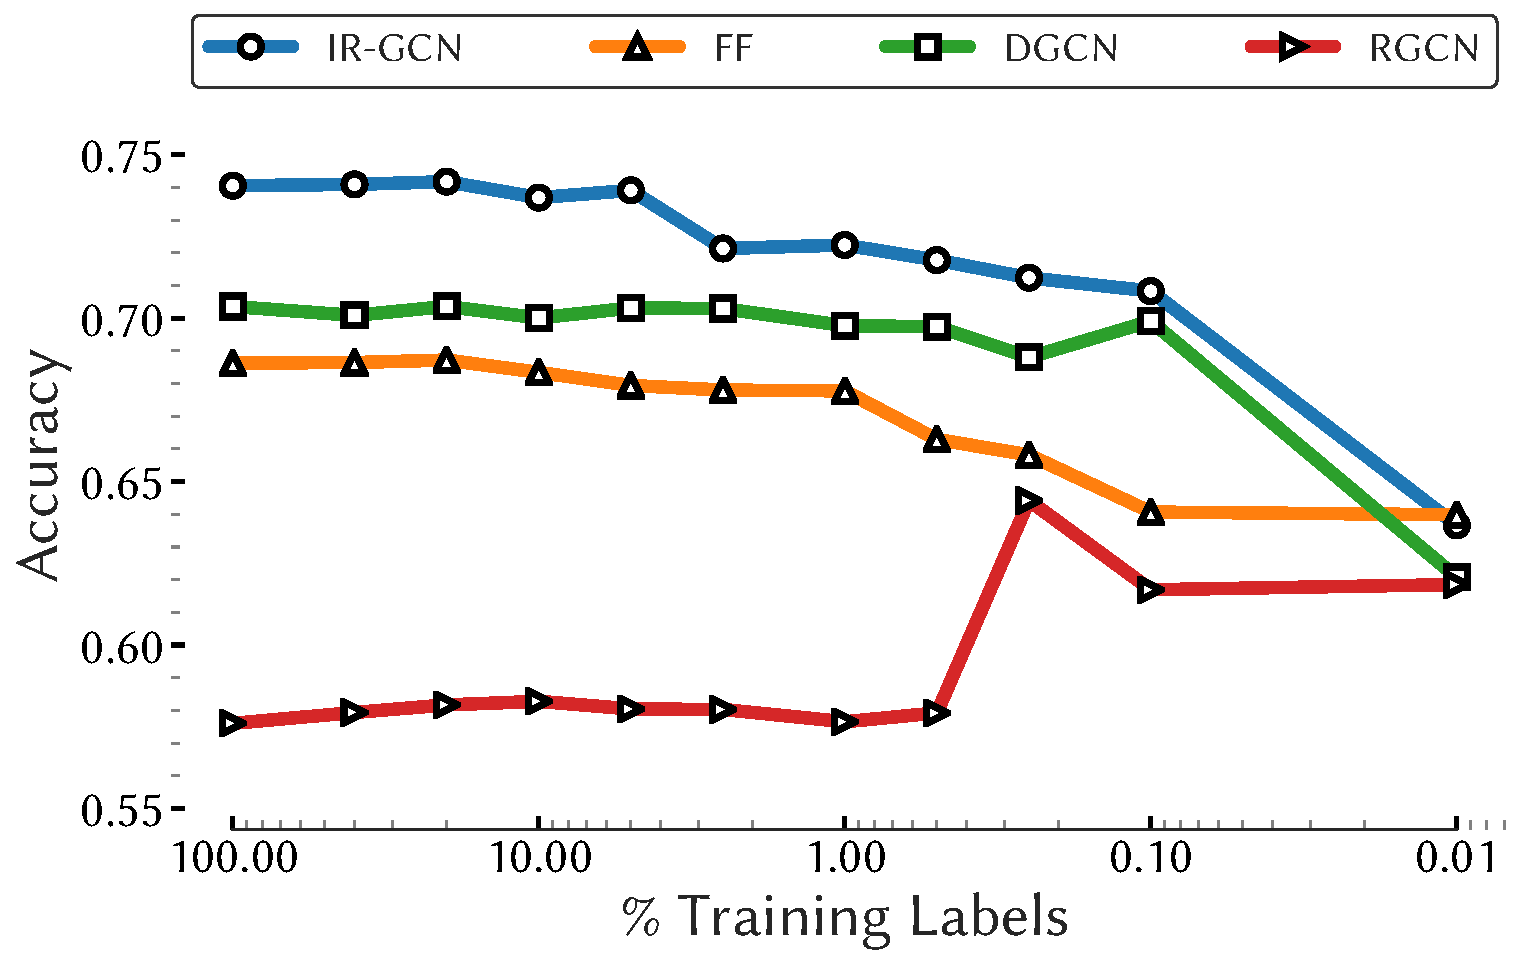
\includegraphics[scale=0.5]{figures/sparsity_acc_physics.pdf}
  \caption{\label{fig:labelsparsity} Change in accuracy with varying training label rates for Physics StackExchange. Our model is more robust to label sparsity than other relation ensemble approaches. RGCN works better with fewer labels as contrastive relation introduces noise in the model. At extreme sparsity, all approaches converge to the same value indicating random selection.}
\end{figure}
Graph Convolution Networks are robust to label sparsity as they exploit graph structure and are thus heavily used for semi-supervised settings. Figure \ref{fig:labelsparsity} shows the change in accuracy for Physics StackExchange from the Science category at different training label rates. Even though our graph contains disconnected cliques, IR-GCN still preserves robustness to label sparsity.
In contrast, the accuracy of the FeedForward model declines sharply with less label information. Performance of DualGCN remains relatively stable while Relational GCN's performance increases with a decrease in label rate. Relational GCN assumes each view to be of similarity relation, and thus, adding contrastive relation introduces noise in the model. However, as the training labels become extremely sparse, the training noise decreases that leads to a marked improvement in the model. In the case of an extremely low label rate of 0.01\%, all approaches converge to the same value, which is the expectation of theoretically random selection. We also obtained similar results for the other four StackExchange communities.


\subsection{Including Textual Features}
Most of the current literature focuses on using textual similarity for Answer Selection. In this section, we compare our proposed IR-GCN model to a popular text-based model~\cite{Tan2015} for answer selection.

\noindent
\textbf{Text Preprocessing}: For this experiment, we first preprocessed the text of both questions and answers.
We first removed all code snippets, HTML tags, stopwords, and URLs from the text of all questions and answers. We then tokenized the text using NLTK tokenizer followed by lemmatization using WordNetLemmatizer and finally converted it into lowercase.

We use torchtext (\url{https://pytorch.org/text/}) to create vocabulary and limit the text of each question and answer to be 250 words long. We initialized the words in the vocabulary using 300-dimensional pre-trained embeddings from Word2vec (\url{https://code.google.com/archive/p/word2vec/}). We randomly initialized words present in the vocabulary but not in word2vec.

We evaluate multiple approaches to test the effectiveness of incorporating textual features for answer selection task.
\noindent
\textbf{QA-LSTM/CNN \cite{Tan2015}} uses a stacked bidirectional LSTM model followed by convolution filters to extract embeddings for the question and answer text separately. Answers are then classified according to the cosine similarity of learned question and answer embedding.

Specifically, in this baseline, we use a biLSTM model with a hidden dimension = 300, followed by 50 1D convolutional filters with a kernel size of 3. We then compute the final embeddings by applying 1D max-pooling on the output of the convolution layer. We also used Tanh nonlinearity and a dropout of 0.3 on the final embeddings. We finally use these embeddings to compute a cosine similarity score between a question and its answers. This score is used to rank the candidate answers for evaluation. We implemented the baseline in Pytorch.

\noindent
\textbf{Textual Similarity (T-GCN)} We create a \textit{SimilarContrast} view that connects answers authored by a user where her answer is significantly similar (dissimilar) to the question than other competing answers. We used cosine similarity on the learned question and answer embedding from the QA-LSTM/CNN approach as the similarity function.

Specifically, we extract the updated embeddings of the question and answer text from the learnt QA-LSTM model. We then compute cosine similarity between the embeddings of each question and its answers.
We then connect answers authored by a specific user, where the difference in cosine similarity of the answer with the other competing answers is greater than margin $\lambda$. Specifically, if the user authors answers $a, a'$ to questions $q, q'$, we create a link between $a$ and $a'$ if
\begin{align}
 \lvert C_{q,a} - C_{q, b} \rvert &> \lambda; \forall b \in \mathcal{A}_(q) \\
 \lvert C_{q,a'} - C_{q, c} \rvert &> \lambda; \forall c \in \mathcal{A}_(q')
\end{align}
where $C_{q,a}$ is the cosine similarity of the answer $a$ with respect to question $q$. Similarly, a link is created for the opposite case when difference is less than $-\lambda$. In our experiments, we assign $\lambda = 0.4$. The hypothesis is that irrelevant(dissimilar) answers will more likely be rejected and vice versa.

\noindent
\textbf{IR-GCN + T-GCN} extends our proposed model to also include the Textual Similarity as the third \textit{SimilarContrast} view in addition to Arrival and TrueSkill Similarity.

\begin{table}[h]
  \centering
  \begin{tabular}{l | S[round-mode=places,round-precision=2]S[round-mode=places,round-precision=2]S[round-mode=places,round-precision=2]S[round-mode=places,round-precision=2]S[round-mode=places,round-precision=2]}
    \toprule
    {Method} &
      {Tech} &
      {Culture} &
      {Life} &
      {Sci} &
      {Business}\\
      \midrule
    QA-LSTM/CNN\cite{Tan2015} & 66.49 & 71.70  & 69.42 & 62.91 & 72.55 \\
    FF~\cite{JendersKN16} & 68.30 & 73.35 & 76.57 & 67.40 & 75.76 \\
    C-GCN & 71.23 & 75.90 & 78.71 & 72.99 & 76.85 \\
    T-GCN & 69.25 & 73.77 & 76.39 & 67.79 & 77.08\\
    IR-GCN & 73.87 & 78.74 & 81.60 & 74.68 & 80.56 \\
    IR-GCN + T-GCN & 73.89 & 78.00  & 81.07 & 74.49 & 78.86\\
    \bottomrule
  \end{tabular}
  \caption{\label{tab:text} 5-fold Accuracy comparison of text-based baseline and textual similarity GCN with IR-GCN.}
\end{table}

In general, the text-based baseline, QA-LSTM, performs worse than even reflexive GCN, as shown in Table \ref{tab:text}. Note that reflexive GCN employs a feedforward model on the activity and user features used in our experiments. This worse performance is surprising as most of the current literature focuses on textual features for the task. Our results indicate that non-textual features are useful too for answer selection task on StackExchange communities.

Textual Similarity GCN performs better than QA-LSTM and Reflexive GCN. Even though we use the output of QA-LSTM to construct the graph for T-GCN, the graph improves performance as it connects answers across questions. However, adding the T-GCN view in our proposed IR-GCN model decreases the performance slightly. One possible explanation could be that similar contrast views based on user features (Arrival similarity and TrueSkill similarity) are not compatible with views based on textual features.

\begin{table}[h]
  \centering
  \begin{tabular}{l | S[round-mode=places,round-precision=2]S[round-mode=places,round-precision=2]S[round-mode=places,round-precision=2]S[round-mode=places,round-precision=2]S[round-mode=places,round-precision=2]}
    \toprule
    {Method} &
      {Tech} &
      {Culture} &
      {Life} &
      {Sci} &
      {Business}\\
      \midrule
    QA-LSTM/CNN\cite{Tan2015} & 66.49 & 71.70 & 69.42 & 62.91 & 72.55 \\
    FF~\cite{JendersKN16} & 66.00 & 72.22 & 69.85 & 63.63 & 75.57 \\
    C-GCN & 66.19 & 72.45 & 70.23 & 63.89 & 75.71 \\
    CT-GCN & 66.06 & 72.35 & 71.88 & 64.14 & 75.69 \\
    IR-GCN & 66.56 & 72.92 & 72.54 & 65.11 & 75.95 \\
    IR-GCN + T-GCN & 66.49 & 73.17 & 72.85 & 65.29 & 75.86 \\
    \bottomrule
  \end{tabular}
  \caption{\label{tab:textfeature} 5-fold Accuracy comparison of text-based baseline and textual similarity GCN with learnt text embeddings as features in the GCN.}
\end{table}

We further replaced our activity-based features with the learned embeddings obtained after training the QA-LSTM/CNN~\cite{Tan2015} model as the node features. We observed that the performance of all approaches went down slightly when using textual features only (Table \ref{tab:textfeature}). As we noted before, GCNs aggregate features among the neighbors. In our similar contrast views, it is not favorable to aggregate textual features among the neighbors as it connects answers catering to different questions. Thus, aggregating textual features creates noise in the model leading to worse performance \footnote{We also experimented with concatenating textual features with the original features used in the previous experiments. However, the performance was still a little worse than the results with only original features.}.


\subsection{Contrastive GCN Analysis}
\label{ref:analysis}
The ability of neural networks to perform classification in sparse high-dimensional manifolds has been studied in past work, especially in the context of adversarial learning \cite{lu2017safetynet}. We employ the ReLU activation function in our convolution layers and study the outputs of the $k$th layer, i.e., embeddings with k-order locality. This transformation breaks the input space into cells with smooth gradients within each cell, at whose boundaries the piecewise linear function changes (i.e., the likelihood of the two classes of answers).

We ask a specific question in the context of our Contrastive GCN. \emph{What is the impact of the layerwise discriminative magnification induced by our formulation?} Discriminative magnifications result in improved separability of the two classes in the later convolving layers, an effect we earlier demonstrated with a sample network in \cref{fig:contrast}. This positively impacts the ability of the model to explain the observed data points (i.e., create p-domains that are well aligned with the contrastive samples provided) and improve the generalizability of the learned model to unseen data points. However, it is crucial to maintain sufficient regularization with weight decay to prevent sparse regions exhibiting sharp gradients that could affect model performance.

The capacity of our model can also be quantified in terms of the VC dimension of the aggregated classifier against the individual learners. Gradient boosting with multiple relation learners (each of which captures a specific aspect of node locality via graph convolution on the induced relations) could boost the capacity of the joint model, enabling better generalization and a more accurate fit in the data manifold (i.e., higher capacity to fit regions to fine distinctions).

Let us denote the upper bound of the VC dimension or capacity of each individual learner as D (If the individual learners do not have identical capacity, the minimum can be used to compute a lower bound on the aggregated learner capacity). Then the gradient boosted learner with T classifiers has a bound on it's capacity~\cite{shalev2014understanding} given by,
\begin{equation}
\mathcal{VC}_{Agg}  = T \times (D+1) \times(3 \log(T.(D+1))+2)
\label{vcdim}
\end{equation}

Thus we identify two potential reasons for our performance gains, first the discriminative magnification effect that also supports the strong individual performance of the contrast view, and second the gain in capacity from boosting, which could explain its advantage over competing aggregation methods.
